\documentclass[tikz,border=20pt]{standalone}
\usepackage{amsmath}
\usetikzlibrary{positioning, arrows.meta}

\begin{document}
	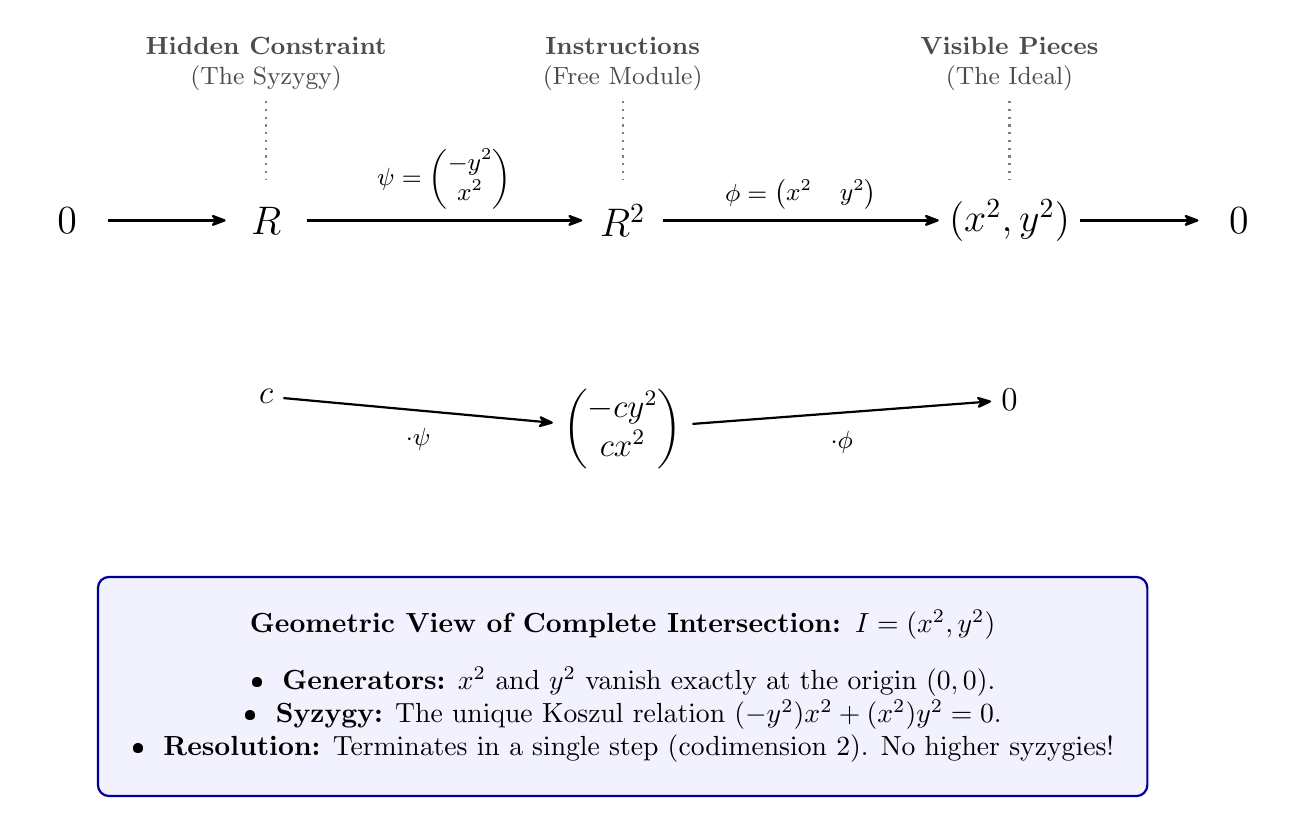
\begin{tikzpicture}[
		>={Stealth[round]}, thick,
		module/.style={font=\Large\bfseries, minimum size=1cm},
		map/.style={->, font=\small},
		element/.style={font=\large},
		note/.style={font=\small\color{black!70}, align=center}
		]
		
		% --- Exact Sequence ---
		\node[module] (0L) {$0$};
		\node[module, right=1.5cm of 0L] (R) {$R$};
		\node[module, right=3.5cm of R] (R2) {$R^2$};
		\node[module, right=3.5cm of R2] (I) {$(x^2,y^2)$};
		\node[module, right=1.5cm of I] (0R) {$0$};
		
		\draw[map] (0L) -- (R);
		\draw[map] (R) -- node[above] {$\psi = \begin{pmatrix} -y^2 \\ x^2 \end{pmatrix}$} (R2);
		\draw[map] (R2) -- node[above] {$\phi = \begin{pmatrix} x^2 & y^2 \end{pmatrix}$} (I);
		\draw[map] (I) -- (0R);
		
		% --- Annotations above ---
		\node[note, above=1cm of R] (note1) {\textbf{Hidden Constraint}\\(The Syzygy)};
		\node[note, above=1cm of R2] (note2) {\textbf{Instructions}\\(Free Module)};
		\node[note, above=1cm of I] (note3) {\textbf{Visible Pieces}\\(The Ideal)};
		
		\draw[dotted, gray] (note1) -- (R);
		\draw[dotted, gray] (note2) -- (R2);
		\draw[dotted, gray] (note3) -- (I);
		
		% --- Elements below ---
		\node[element, below=1.5cm of R] (e1) {$c$};
		\node[element, below=1.5cm of R2] (e2) {$\begin{pmatrix} -cy^2 \\ cx^2 \end{pmatrix}$};
		\node[element, below=1.5cm of I] (e3) {$0$};
		
		\draw[|->, map] (e1) -- node[below=0.1cm] {$\cdot \psi$} (e2);
		\draw[|->, map] (e2) -- node[below=0.1cm] {$\cdot \phi$} (e3);
		
		% --- Geometry Box ---
		\node[draw=blue!60!black, fill=blue!5, rounded corners, align=center, inner sep=12pt, below=4cm of R2] (geo) {
			\textbf{Geometric View of Complete Intersection: $I = (x^2, y^2)$} \\[0.3cm]
			\textbullet~ \textbf{Generators:} $x^2$ and $y^2$ vanish exactly at the origin $(0,0)$.\\
			\textbullet~ \textbf{Syzygy:} The unique Koszul relation $(-y^2)x^2 + (x^2)y^2 = 0$.\\
			\textbullet~ \textbf{Resolution:} Terminates in a single step (codimension 2). No higher syzygies!
		};
		
	\end{tikzpicture}
\end{document}